% !TEX program = pdflatex
\documentclass[aspectratio=169, 10pt]{beamer}

% ── Theme ─────────────────────────────────────────────────────────────────────
\usetheme{metropolis}
\usepackage{appendixnumberbeamer}
\usepackage{booktabs}
\usepackage{graphicx}
\usepackage{xcolor}
\usepackage{tikz}
\usetikzlibrary{arrows.meta, positioning, shapes.geometric, fit, calc}
\usepackage{amsmath}
\usepackage{amssymb}
\usepackage{adjustbox}

% colours
\definecolor{accent}{HTML}{2980B9}
\definecolor{good}{HTML}{27AE60}
\definecolor{bad}{HTML}{E74C3C}
\definecolor{neutral}{HTML}{F39C12}
\setbeamercolor{frametitle}{bg=accent!90!black}
\setbeamercolor{progress bar}{fg=accent}

% figure path: supports compiling from repo root or docs/presentation_slides
\graphicspath{{results/}{../../results/}}

\title{DQN \& DDQN for Automated Stock Trading}
\subtitle{Implementation, Iterative Improvements \& Results}
\author{Yufan Zhu \and Rutwik Shrikant Dharanappagoudar}
\date{\today}

\begin{document}

\maketitle

% ---------------------------------------------------------------------
% YUFAN SECTION
% ---------------------------------------------------------------------
\section{Yufan: Data, Environment \& Initial System}

\begin{frame}[shrink=5]{Yufan --- Data Pipeline \& Feature Engineering}
\begin{columns}[T]

\begin{column}{0.55\textwidth}
\vspace{-0.4em}
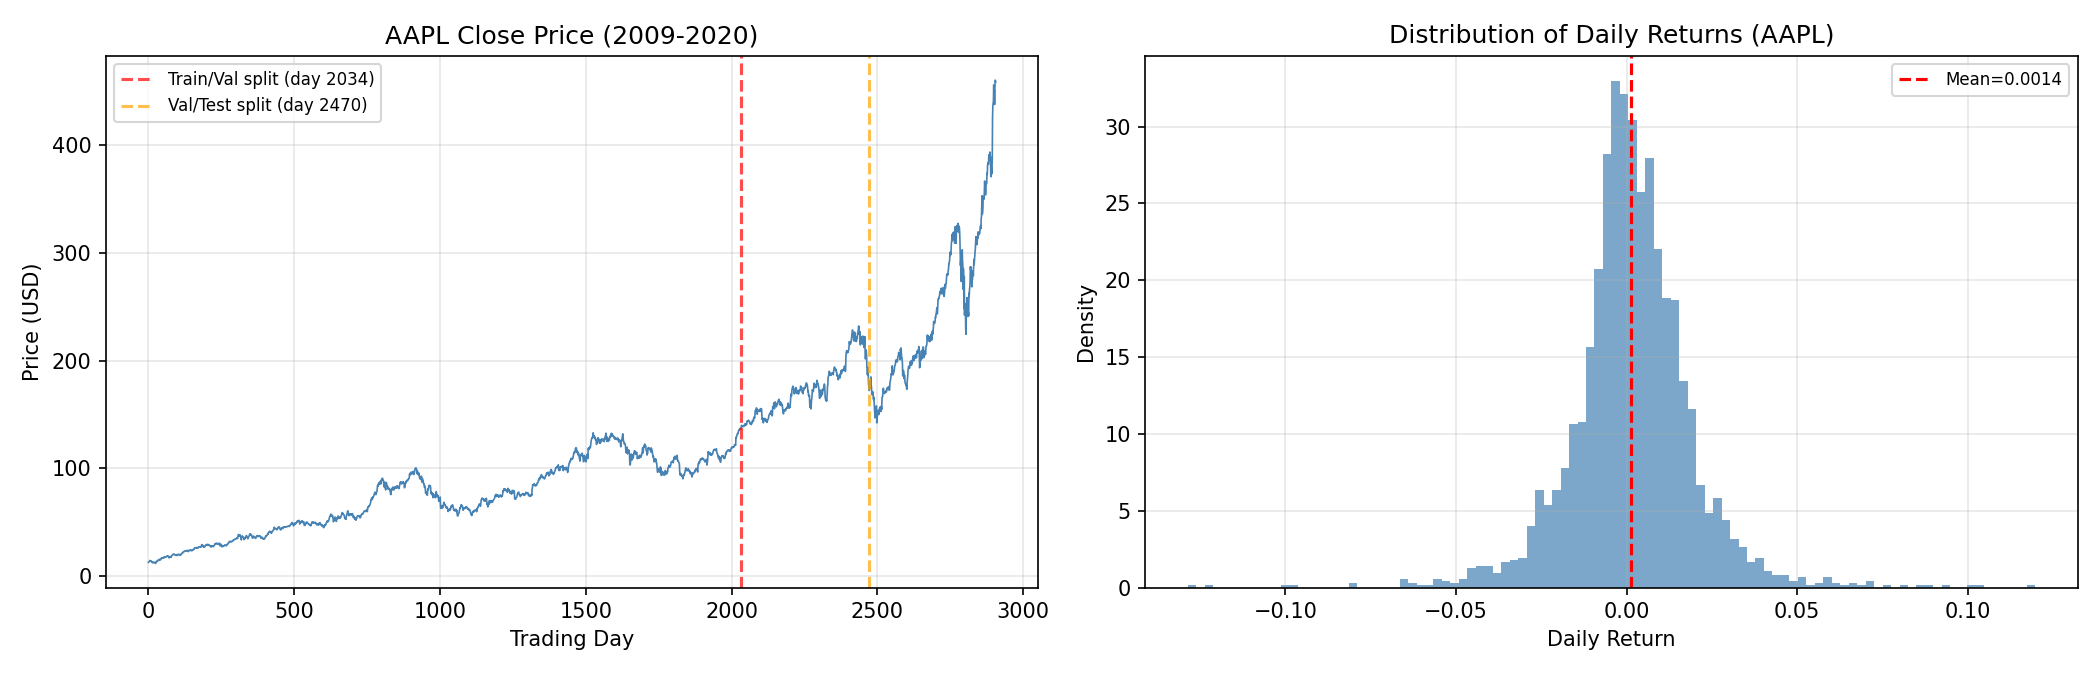
\includegraphics[width=\linewidth]{data_exploration.png}

\vspace{0.2em}
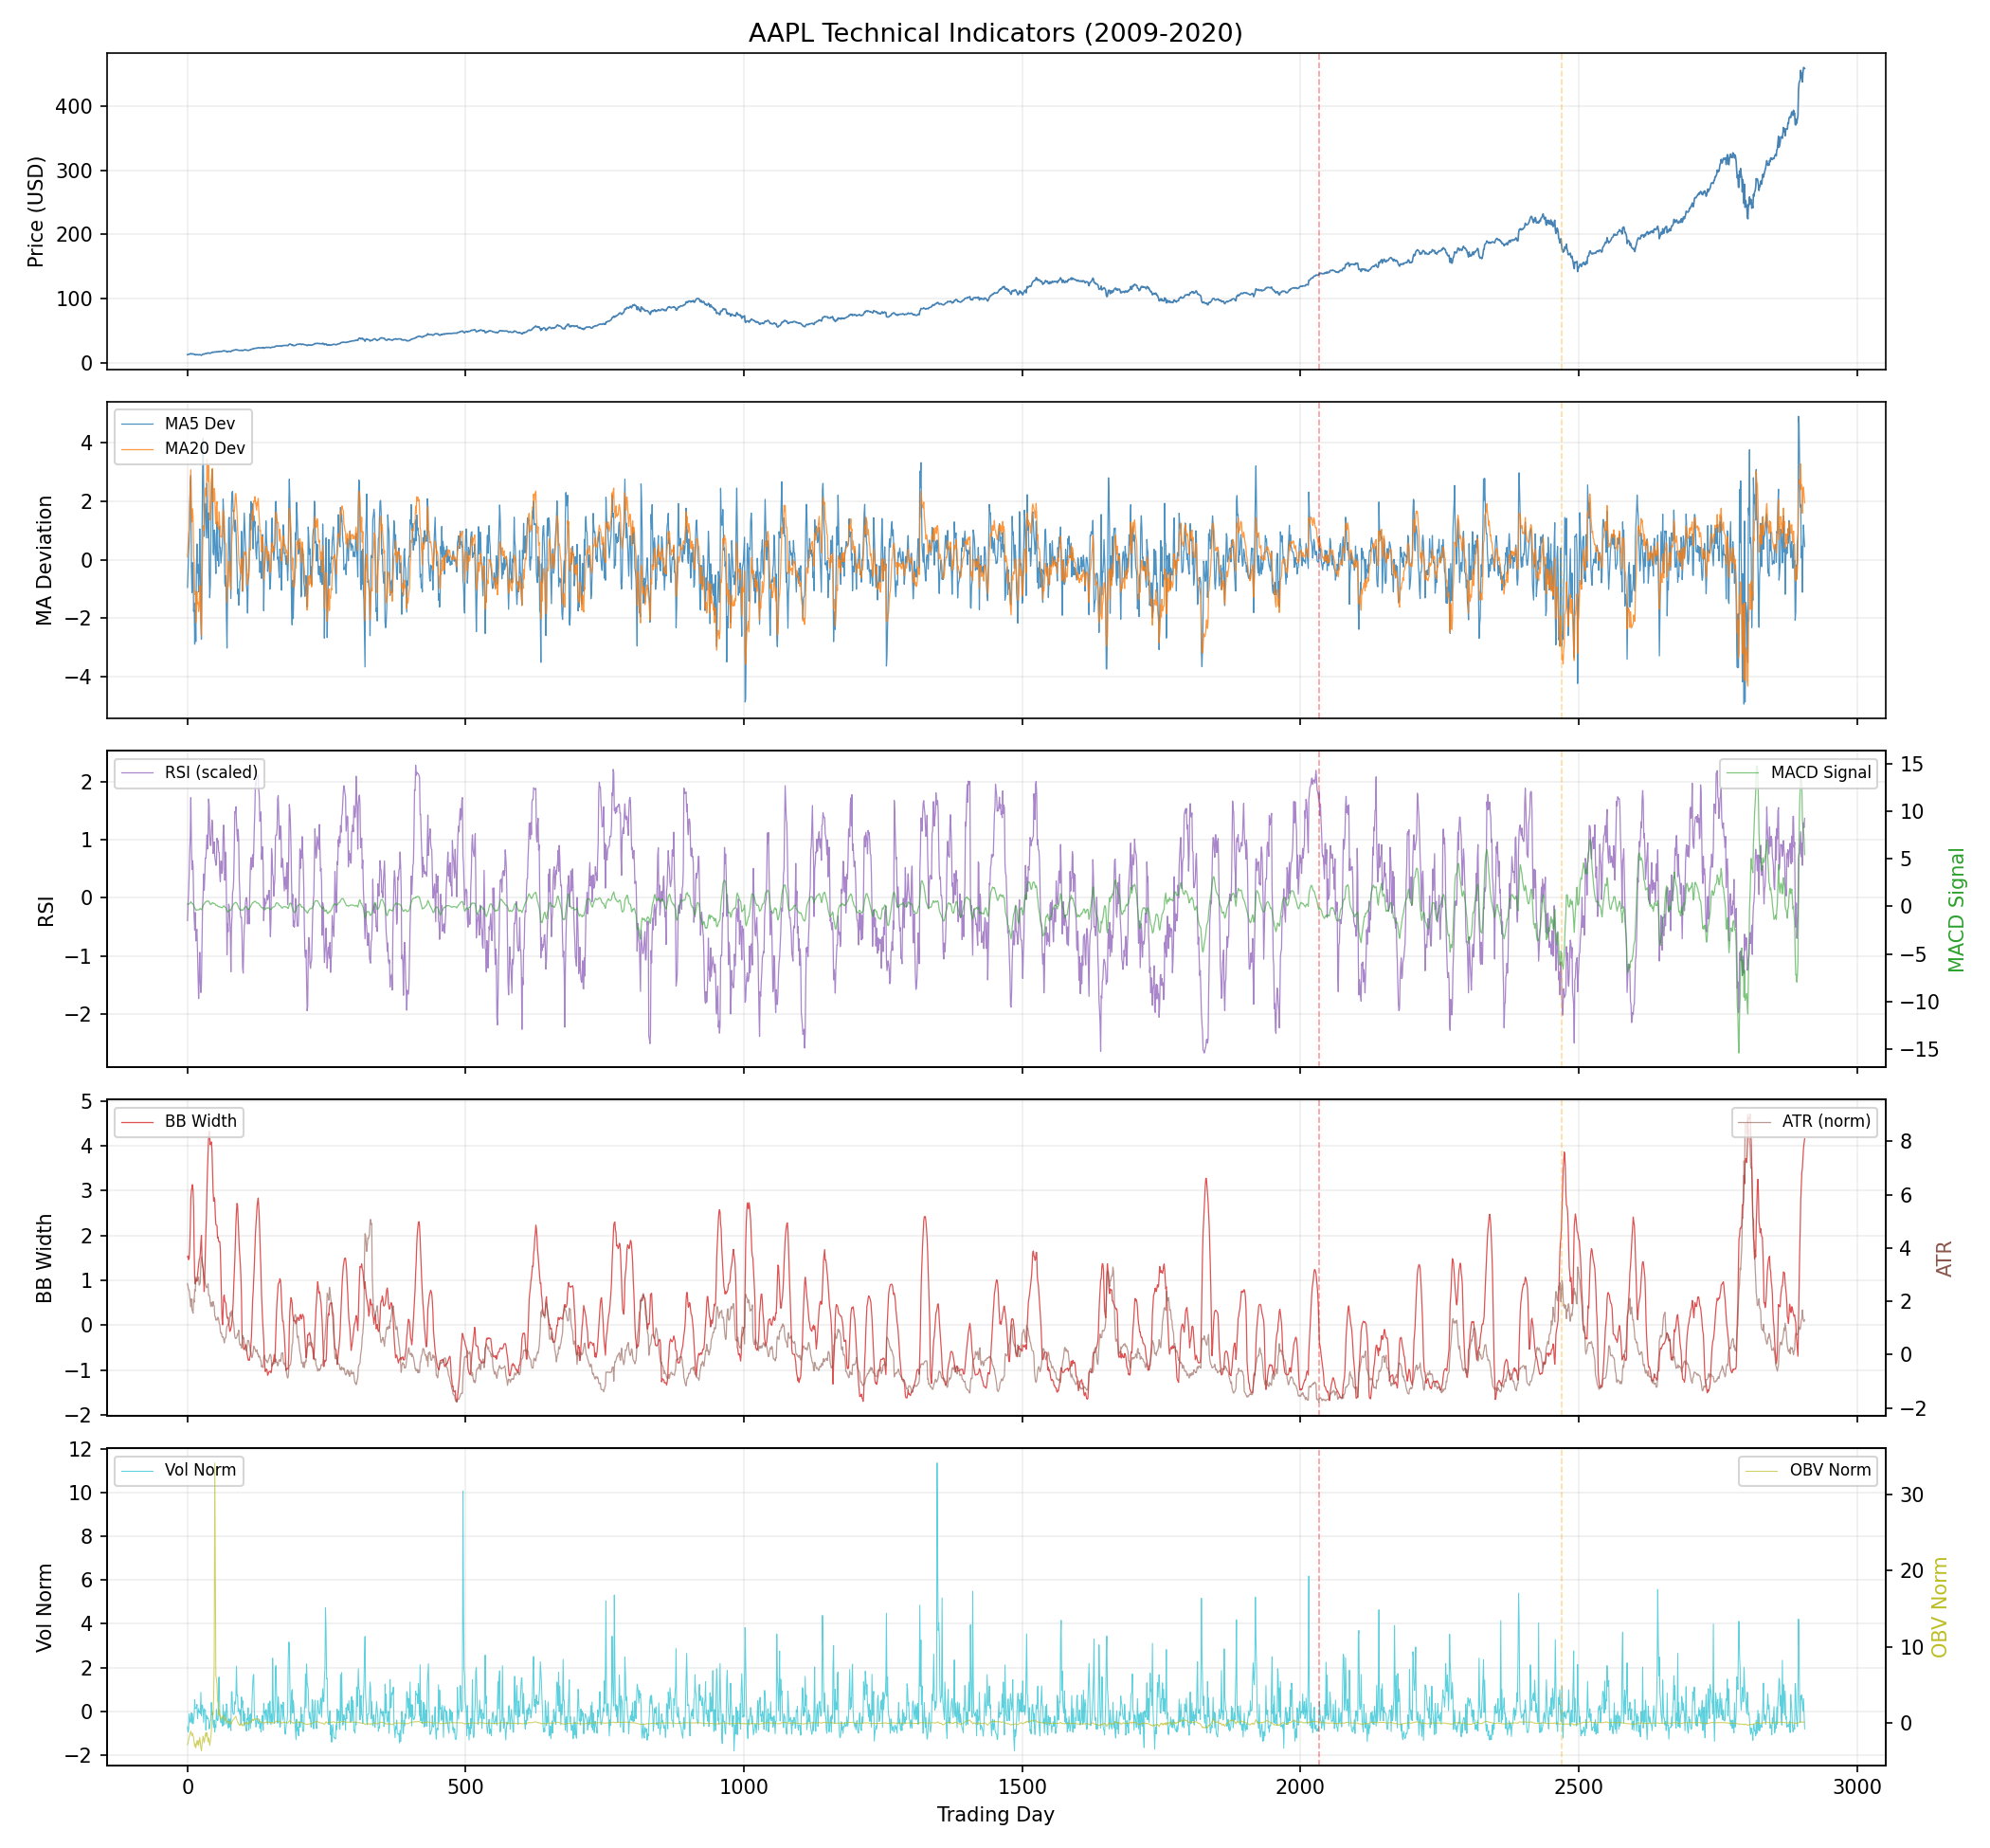
\includegraphics[width=\linewidth, height=2.5cm, keepaspectratio]{technical_indicators.png}

\vspace{-0.1em}
{\tiny AAPL is split chronologically into train, validation and test periods; all normalisation uses train-set statistics only.}
\end{column}

\begin{column}{0.43\textwidth}
\vspace{-0.4em}
{\scriptsize \textbf{Reproducible market-data pipeline}}

\vspace{0.2em}
{\tiny
\begin{itemize}\setlength\itemsep{3pt}
  \item Kaggle \texttt{alincijov/trading} loaded via \texttt{kagglehub}.
  \item DJIA ticker subset with AAPL case study.
  \item Chronological 70/15/15 train-val-test split.
  \item Raw returns preserved for rewards and portfolios.
\end{itemize}
}

\vspace{0.3em}
{\scriptsize \textbf{Nine engineered indicators}}

\vspace{0.2em}
{\tiny
\begin{tabular}{@{}ll@{}}
\toprule
\textbf{Group} & \textbf{Features} \\
\midrule
Trend & Return, MA5 dev., MA20 dev. \\
Momentum & RSI-14, MACD \\
Volatility & Bollinger width, ATR \\
Volume & Normalised volume, OBV \\
\bottomrule
\end{tabular}}

\vspace{0.35em}
{\tiny \textcolor{accent}{\textbf{Goal:}} give each agent the same clean, leakage-safe state representation before comparing algorithms.}
\end{column}
\end{columns}
\end{frame}

\begin{frame}[shrink=5]{Yufan --- Trading Environment \& Evaluation}
\begin{columns}[T]

\begin{column}{0.52\textwidth}
\vspace{-0.2em}
\begin{center}
\resizebox{0.98\linewidth}{!}{%
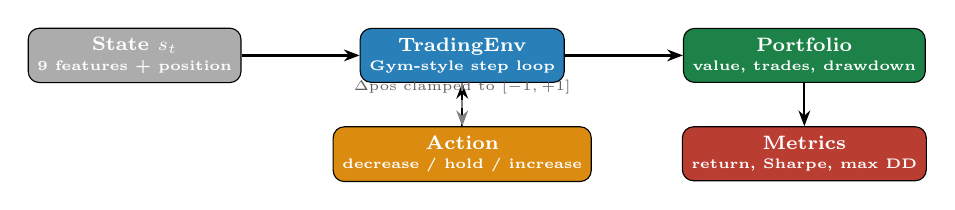
\begin{tikzpicture}[
    node distance=0.55cm and 0.9cm,
    block/.style={draw, rounded corners, minimum width=2.1cm, minimum height=0.55cm,
                  font=\scriptsize\bfseries, text=white, align=center},
    arrow/.style={-{Stealth[length=2mm]}, thick},
    lbl/.style={font=\tiny, text=gray!75!black}
]
  \node[block, fill=gray!65] (state) {State $s_t$\\[-1pt]{\tiny 9 features + position}};
  \node[block, fill=accent, right=1.5cm of state] (env) {TradingEnv\\[-1pt]{\tiny Gym-style step loop}};
  \node[block, fill=neutral!90!black, below=0.55cm of env] (action) {Action\\[-1pt]{\tiny decrease / hold / increase}};
  \node[block, fill=good!75!black, right=1.5cm of env] (portfolio) {Portfolio\\[-1pt]{\tiny value, trades, drawdown}};
  \node[block, fill=bad!80!black, below=0.55cm of portfolio] (metrics) {Metrics\\[-1pt]{\tiny return, Sharpe, max DD}};

  \draw[arrow] (state) -- (env);
  \draw[arrow] (env) -- (portfolio);
  \draw[arrow] (action) -- (env);
  \draw[arrow] (portfolio) -- (metrics);
  \draw[arrow, dashed, gray] (env.south) -- node[above, lbl] {$\Delta$pos clamped to $[-1,+1]$} (action.north);
\end{tikzpicture}}
\end{center}

\vspace{0.4em}
{\tiny
\begin{align*}
V_t &= V_{t-1}\bigl(1 + \mathrm{pos}_t \tilde r_t - c_t \mathbf{1}[\Delta\mathrm{pos}\neq 0]\bigr)\\[-2pt]
r_t &= \log(V_t/V_{t-1}) + \lambda \min(0, \mathrm{drawdown}_t)
\end{align*}
}
\end{column}

\begin{column}{0.46\textwidth}
\vspace{-0.4em}
{\scriptsize \textbf{Environment design choices}}

\vspace{0.2em}
{\tiny
\begin{itemize}\setlength\itemsep{3pt}
  \item Positions: short, flat, long.
  \item Actions move position by one step.
  \item Transaction cost: 10 bps per position change.
  \item Drawdown penalty discourages fragile portfolios.
  \item Full portfolio history tracked every episode.
\end{itemize}
}

\vspace{0.2em}
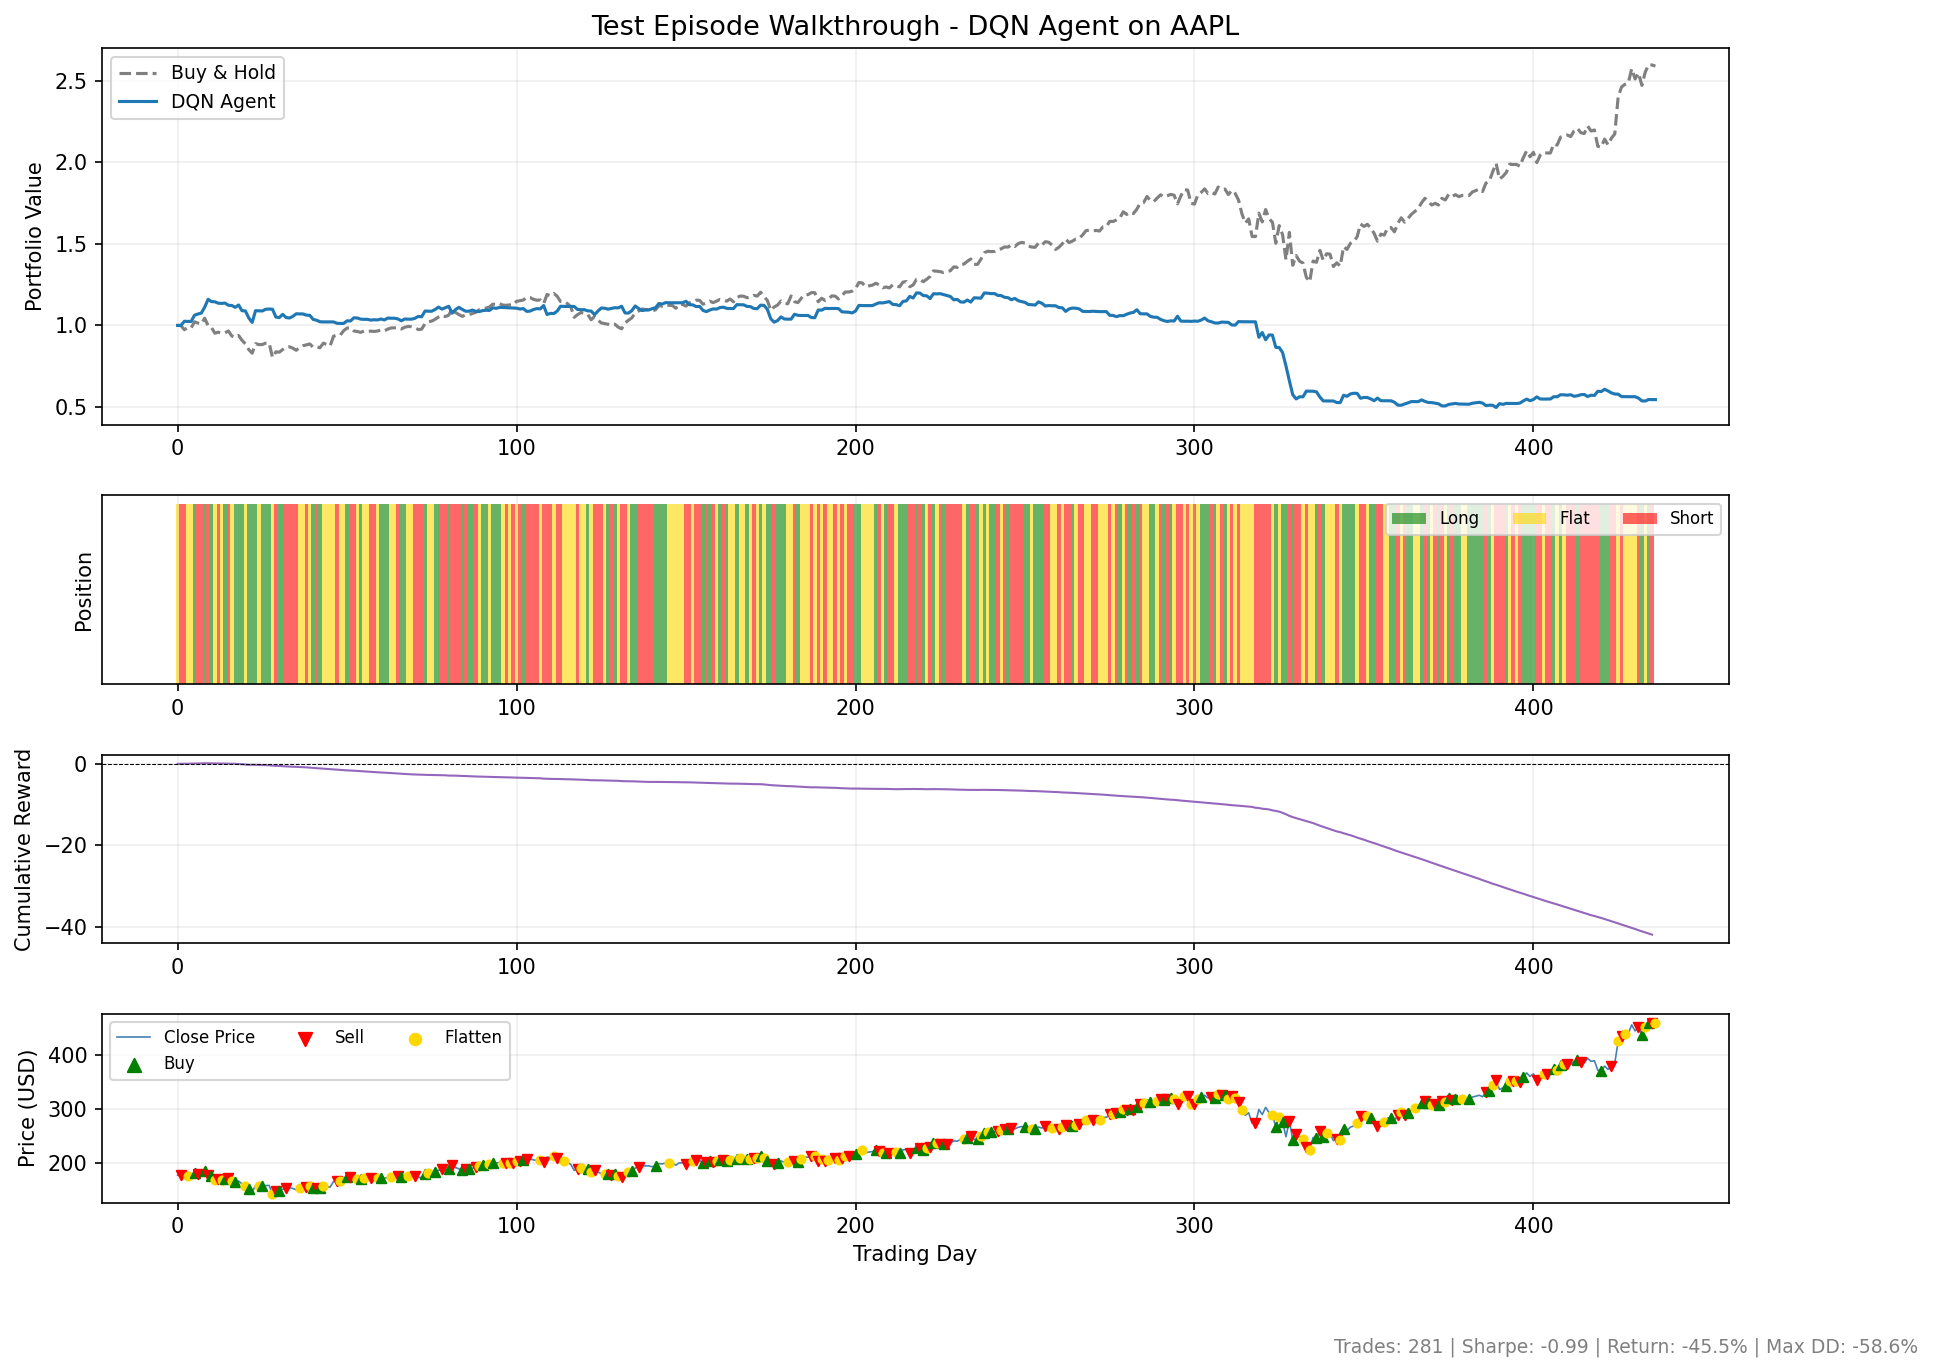
\includegraphics[width=\linewidth, height=3.2cm, keepaspectratio]{episode_walkthrough.png}

\vspace{-0.1em}
{\tiny The walkthrough view links actions to portfolio value, cumulative reward and buy/sell timing.}
\end{column}
\end{columns}
\end{frame}

\begin{frame}[shrink=5]{Yufan --- Initial Agents, Baselines \& Report Assets}
\begin{columns}[T]

\begin{column}{0.48\textwidth}
\vspace{-0.3em}
{\scriptsize \textbf{Initial from-scratch system}}

\vspace{0.2em}
{\tiny
\begin{itemize}\setlength\itemsep{3pt}
  \item Built the first complete codebase.
  \item Implemented \texttt{QNetwork}, replay buffer and target network.
  \item Added DQN/DDQN training and evaluation loops.
  \item Added Random Forest baseline with 200 trees.
  \item Produced data/training figures and appendix material.
\end{itemize}
}

\vspace{0.35em}
{\tiny
\renewcommand{\arraystretch}{1.15}
\begin{tabular}{@{}p{1.9cm}p{3.9cm}@{}}
\toprule
\textbf{Layer} & \textbf{Yufan output} \\
\midrule
Data & Kaggle download, indicators, splits \\
Env & State, reward, costs, metrics \\
Agents & First DQN/DDQN implementation \\
Baselines & Random Forest comparison \\
Report & Figures, appendix, writing \\
\bottomrule
\end{tabular}}
\end{column}

\begin{column}{0.50\textwidth}
\vspace{-0.4em}
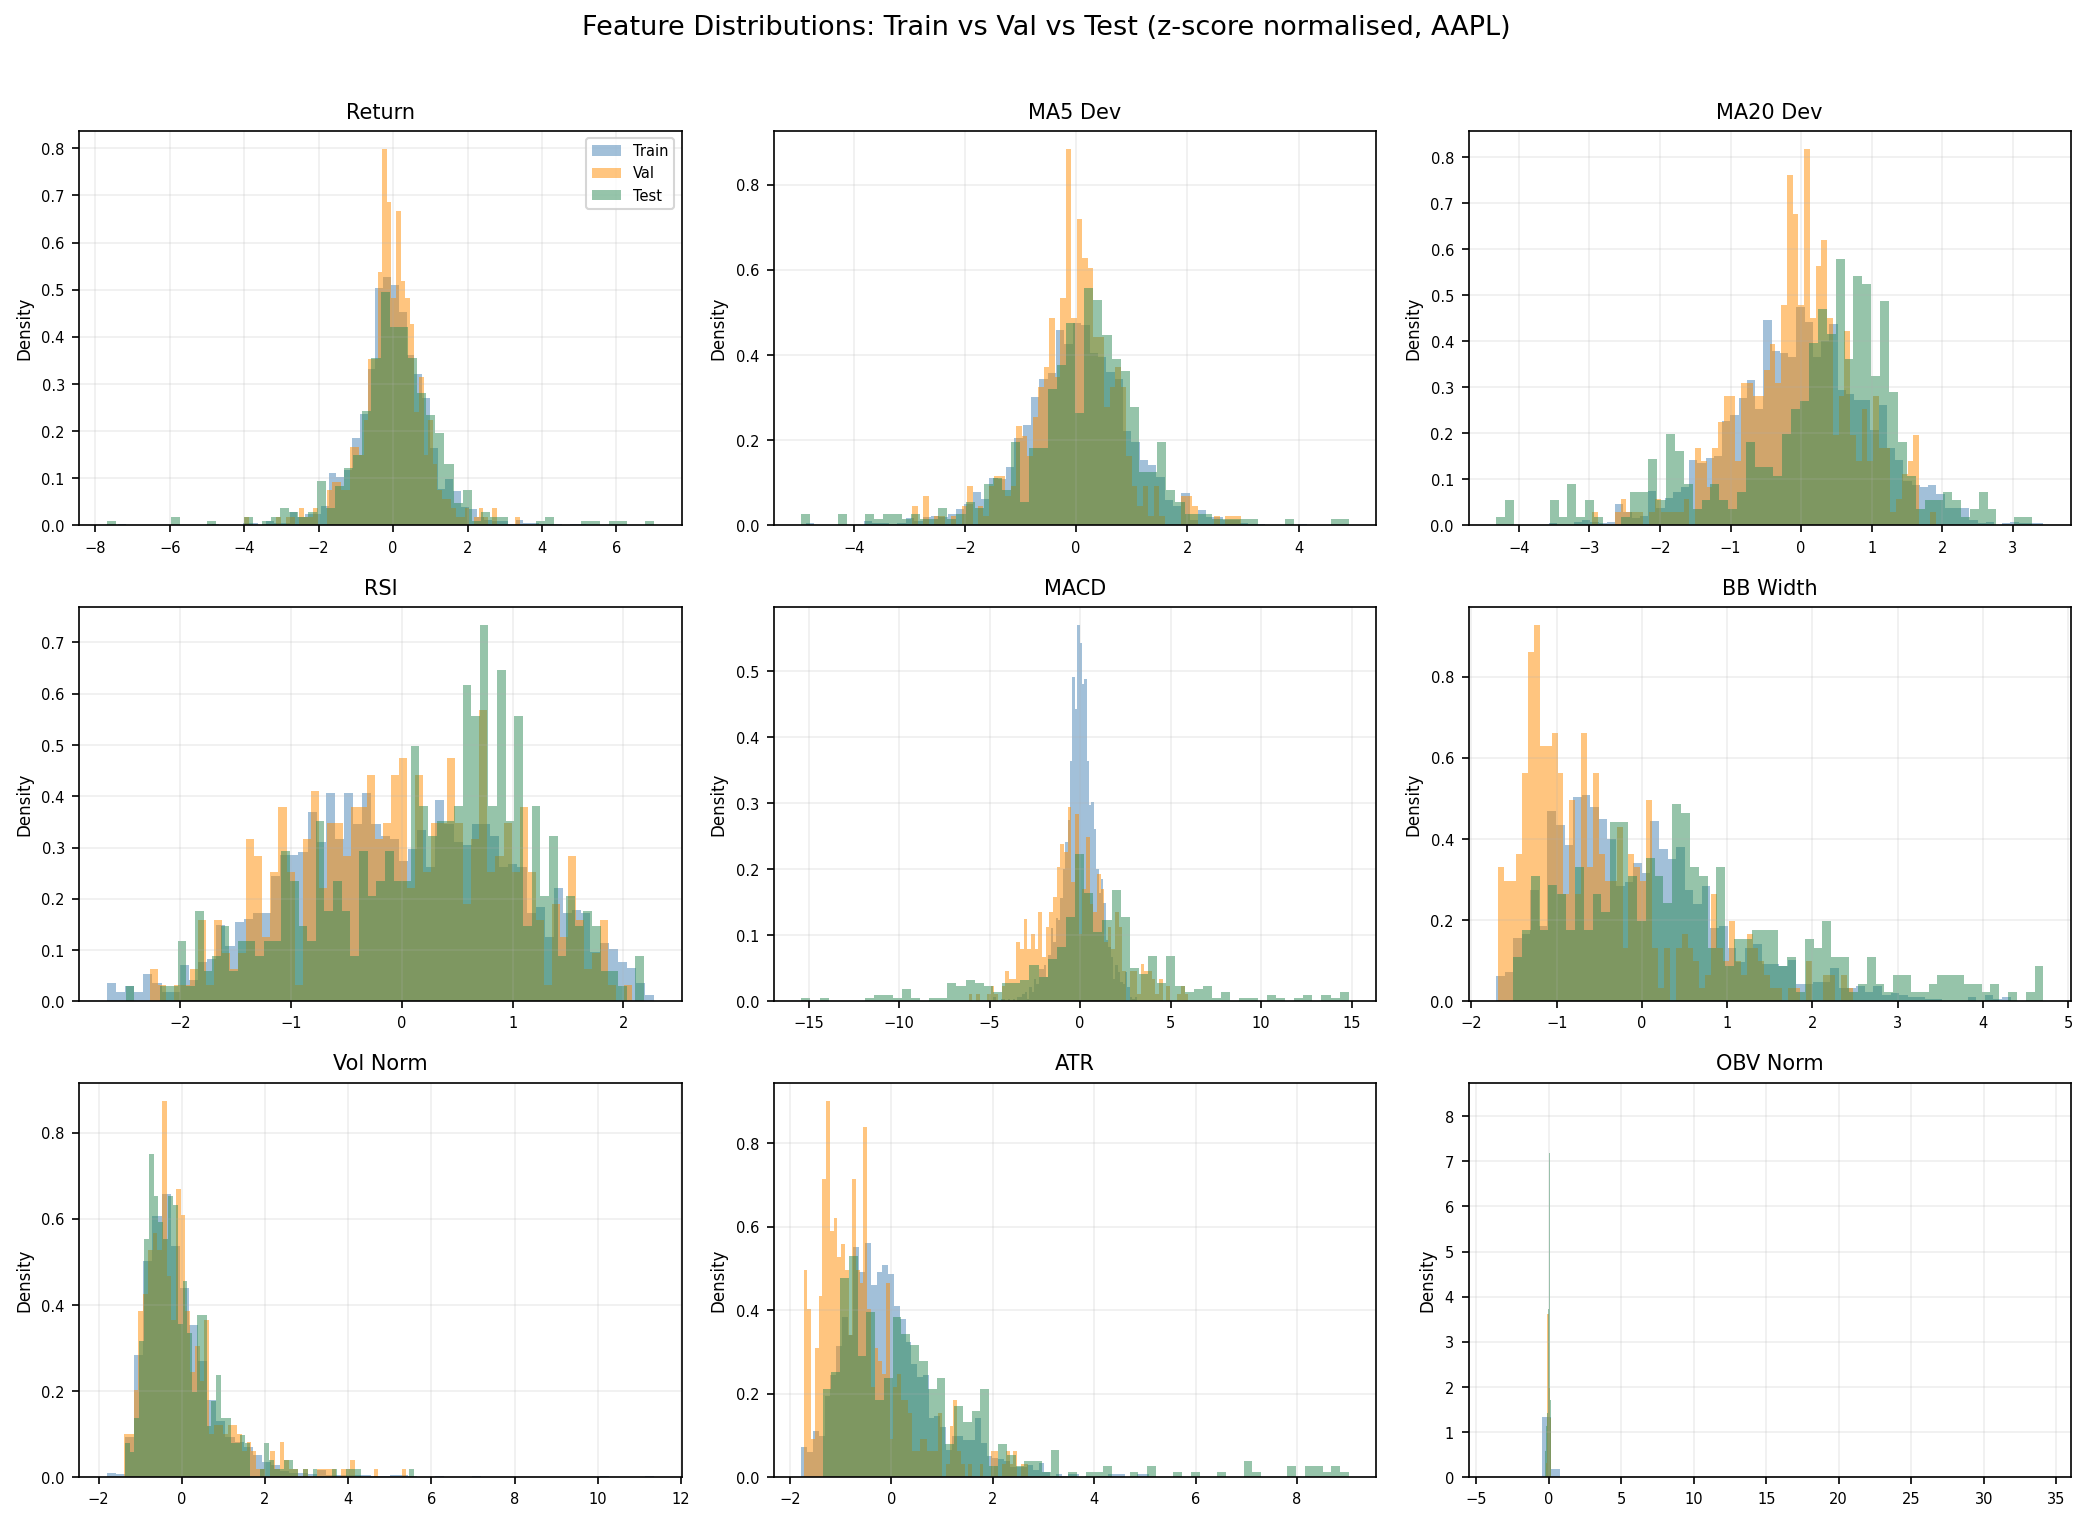
\includegraphics[width=\linewidth, height=3.7cm, keepaspectratio]{feature_distributions.png}

\vspace{0.3em}
\begin{block}{\tiny Why this section matters}
\vspace{-0.4em}
{\tiny
The project depends on a consistent experimental scaffold: same features, same split,
same portfolio accounting and same metrics for every model. This makes later DQN/DDQN
refinements comparable instead of changing the task underneath the agent.
}
\vspace{-0.2em}
\end{block}

\vspace{0.15em}
\begin{block}{\tiny Presentation hand-off}
\vspace{-0.4em}
{\tiny
Yufan establishes the dataset, environment and initial learning system; Rutwik then
focuses on algorithmic refinements, stronger baselines and final result analysis.
}
\vspace{-0.2em}
\end{block}
\end{column}
\end{columns}
\end{frame}

\section{Rutwik: DQN/DDQN Refinements \& Results}

% ══════════════════════════════════════════════════════════════════════════════
% SLIDE 1 — ARCHITECTURE & IMPLEMENTATION
% ══════════════════════════════════════════════════════════════════════════════
\begin{frame}[shrink=5]{DQN \& DDQN --- Architecture \& Implementation}
\begin{columns}[T]

\begin{column}{0.52\textwidth}
\vspace{-0.3em}
\begin{center}
\resizebox{0.92\linewidth}{!}{%
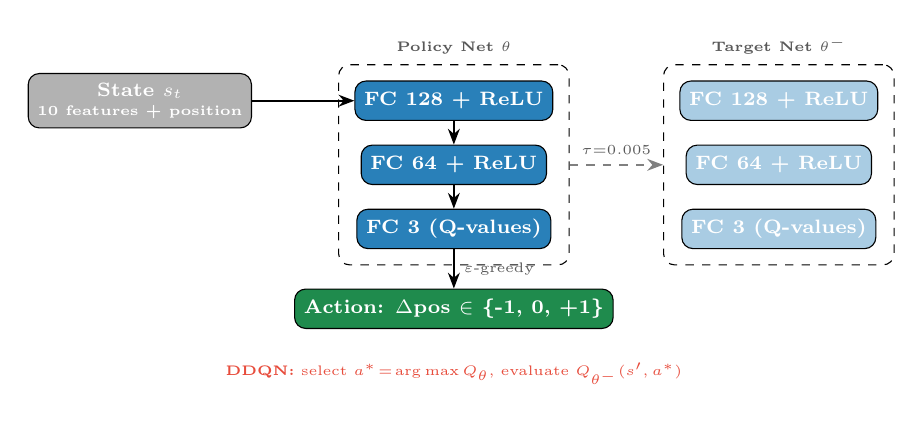
\begin{tikzpicture}[
    node distance=0.5cm and 0.9cm,
    block/.style={draw, rounded corners, minimum width=2.0cm, minimum height=0.5cm,
                  font=\scriptsize\bfseries, text=white, align=center},
    arrow/.style={-{Stealth[length=2mm]}, thick},
    lbl/.style={font=\tiny, text=gray!70!black},
]
    \node[block, fill=gray!60] (state) {State $s_t$\\[-1pt]{\tiny 10 features + position}};
    \node[block, fill=accent, right=1.3cm of state] (fc1) {FC 128 + ReLU};
    \node[block, fill=accent, below=0.3cm of fc1] (fc2) {FC 64 + ReLU};
    \node[block, fill=accent, below=0.3cm of fc2] (fc3) {FC 3 (Q-values)};
    \draw[arrow] (state) -- (fc1);
    \draw[arrow] (fc1) -- (fc2);
    \draw[arrow] (fc2) -- (fc3);
    \node[draw, dashed, rounded corners, inner sep=0.2cm,
          fit=(fc1)(fc2)(fc3), label={[lbl]above:\textbf{Policy Net $\theta$}}] (pnet) {};
    \node[block, fill=accent!40, right=1.6cm of fc1] (tfc1) {FC 128 + ReLU};
    \node[block, fill=accent!40, below=0.3cm of tfc1] (tfc2) {FC 64 + ReLU};
    \node[block, fill=accent!40, below=0.3cm of tfc2] (tfc3) {FC 3 (Q-values)};
    \node[draw, dashed, rounded corners, inner sep=0.2cm,
          fit=(tfc1)(tfc2)(tfc3), label={[lbl]above:\textbf{Target Net $\theta^-$}}] (tnet) {};
    \draw[arrow, dashed, gray] (pnet.east) -- node[above, lbl] {$\tau{=}0.005$} (tnet.west);
    \node[block, fill=good!80!black, below=0.5cm of fc3] (action)
         {Action: $\Delta$pos $\in$ \{-1, 0, +1\}};
    \draw[arrow] (fc3) -- node[right, lbl] {$\varepsilon$-greedy} (action);
    \node[below=0.3cm of action, font=\tiny, text=bad, align=center] {%
      \textbf{DDQN:} select $a^*\!=\!\arg\max Q_\theta$, evaluate $Q_{\theta^-}(s', a^*)$};
\end{tikzpicture}}
\end{center}

\vspace{0.4em}
{\scriptsize
\textbf{DQN}: Replay buffer breaks temporal correlations; target network provides
stable TD targets. Counterfactual replay improves sample efficiency.\\[2pt]
\textbf{DDQN}: Decouples action \emph{selection} (policy net) from \emph{evaluation}
(target net) to reduce overestimation bias.
}
\end{column}

\begin{column}{0.46\textwidth}
\vspace{-0.3em}
{\scriptsize \textbf{10 Technical Features} (z-score normalised):}

\vspace{0.2em}
{\tiny
\begin{tabular}{@{}ll@{}}
\toprule
\textbf{Feature} & \textbf{Signal Type} \\
\midrule
Return, Dev5, Dev20 & Trend / mean-reversion \\
Mom20              & Momentum \\
RSI, MACD          & Oscillator / crossover \\
BB Width, ATR      & Volatility \\
Vol Norm, OBV Norm & Volume flow \\
\bottomrule
\end{tabular}}

\vspace{0.3em}
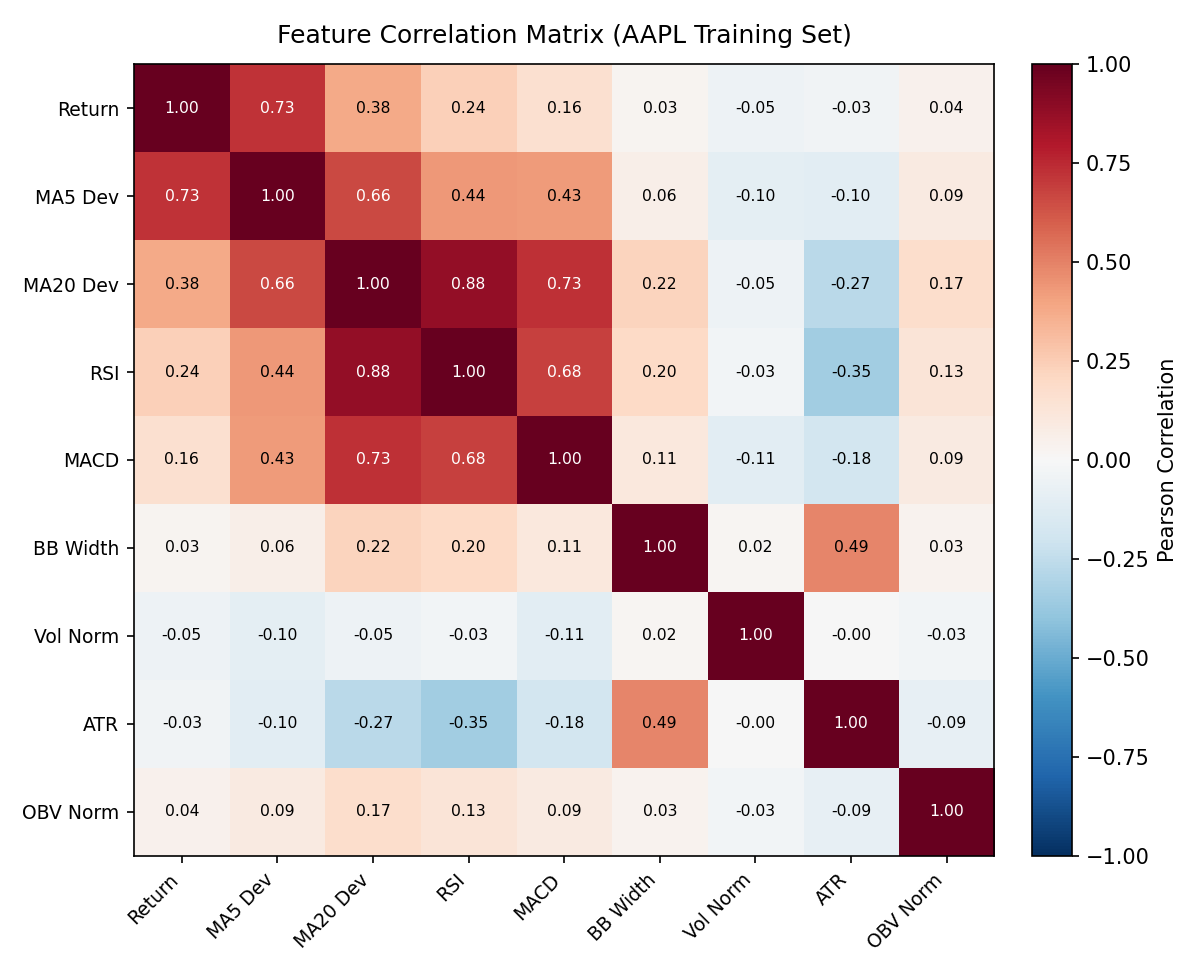
\includegraphics[width=\linewidth, height=4.2cm, keepaspectratio]{feature_correlation.png}

\vspace{0.1em}
{\tiny Volume/volatility indicators are near-uncorrelated with trend indicators, suggesting reduced redundancy and more diverse signals.}
\end{column}
\end{columns}
\end{frame}


% ══════════════════════════════════════════════════════════════════════════════
% SLIDE 2 — ITERATIVE IMPROVEMENTS
% ══════════════════════════════════════════════════════════════════════════════
\begin{frame}[shrink=5]{Iterative Improvements Across Versions}
\begin{columns}[T]

\begin{column}{0.48\textwidth}
\vspace{-0.3em}
{\tiny
\renewcommand{\arraystretch}{1.15}
\begin{adjustbox}{max width=\linewidth}
\begin{tabular}{@{}p{1.4cm}p{1.7cm}p{1.7cm}p{1.7cm}@{}}
\toprule
\textbf{Component} & \textbf{V1 (Initial)} & \textbf{V2 (Core)} & \textbf{V4/HEAD} \\
\midrule
Actions       & Set position        & \textcolor{good}{Delta-based}   & Delta-based \\
Reward        & Raw PnL             & \textcolor{good}{Log-return}    & Log-return \\
$\varepsilon$ & Linear, 1.0$\to$.05 & \textcolor{good}{Exp decay}     & \textcolor{good}{0.2$\to$.02} \\
Target upd.   & Hard (N=100)        & \textcolor{good}{Soft $\tau$=.005} & Soft \\
Loss          & MSE                 & \textcolor{good}{Huber}         & Huber \\
LR / Batch    & 1e-3 / 64           & 5e-4 / 128                     & \textcolor{good}{1e-4} / 128 \\
Buffer        & 10\,k               & 50\,k                          & 50\,k \\
Episodes      & Full dataset        & \textcolor{good}{252d random}   & 252d random \\
Warm start    & ---                 & ---                            & \textcolor{good}{Momentum} \\
Replay        & Standard            & Standard                       & \textcolor{good}{+Counterfact.} \\
\bottomrule
\end{tabular}
\end{adjustbox}}

\vspace{0.4em}
{\tiny \textcolor{good}{\textbf{Green}} = change introduced in that version.}
\end{column}

\begin{column}{0.50\textwidth}
\vspace{-0.3em}
{\scriptsize \textbf{Three most impactful changes:}}

\vspace{0.3em}
\begin{block}{\tiny 1. Reward: Raw PnL $\to$ Log-Return}
\vspace{-0.4em}
{\tiny
$r_t = \log\!\bigl(\tfrac{V_{t+1}}{V_t}\bigr)$ \hfill \textcolor{good}{Scale-invariant, additive}\\[1pt]
Raw PnL was dominated by large price moves; log-return treats gains/losses symmetrically and is additive over time, improving numerical stability for sequential optimisation.
}
\vspace{-0.2em}
\end{block}

\vspace{0.15em}
\begin{block}{\tiny 2. Supervised Warm Start from Momentum Teacher}
\vspace{-0.4em}
{\tiny
Pre-train Q-net via cross-entropy on momentum signal (20d lookback). Builds $(s, a)$ pairs
for \emph{every reachable position} so policy learns entry \& exit. Lower $\varepsilon_0{=}0.2$ preserves pre-trained weights.
}
\vspace{-0.2em}
\end{block}

\vspace{0.15em}
\begin{block}{\tiny 3. TDQN-Style Counterfactual Experience Replay}
\vspace{-0.4em}
{\tiny
For each step, compute \emph{exact} rewards for the 2 actions \textbf{not} taken. Pushes 3$\times$
transitions per step $\to$ $\to$ significantly improves sample efficiency in practice. Possible in our deterministic backtesting environment, where rewards depend only on price data.
}
\vspace{-0.2em}
\end{block}
\end{column}
\end{columns}
\end{frame}


% ══════════════════════════════════════════════════════════════════════════════
% SLIDE 3 — RESULTS & ANALYSIS
% ══════════════════════════════════════════════════════════════════════════════
\begin{frame}{Results \& Analysis (AAPL, 2018--2020 Test Set)}
\begin{columns}[T]

\begin{column}{0.55\textwidth}
\vspace{-0.5em}
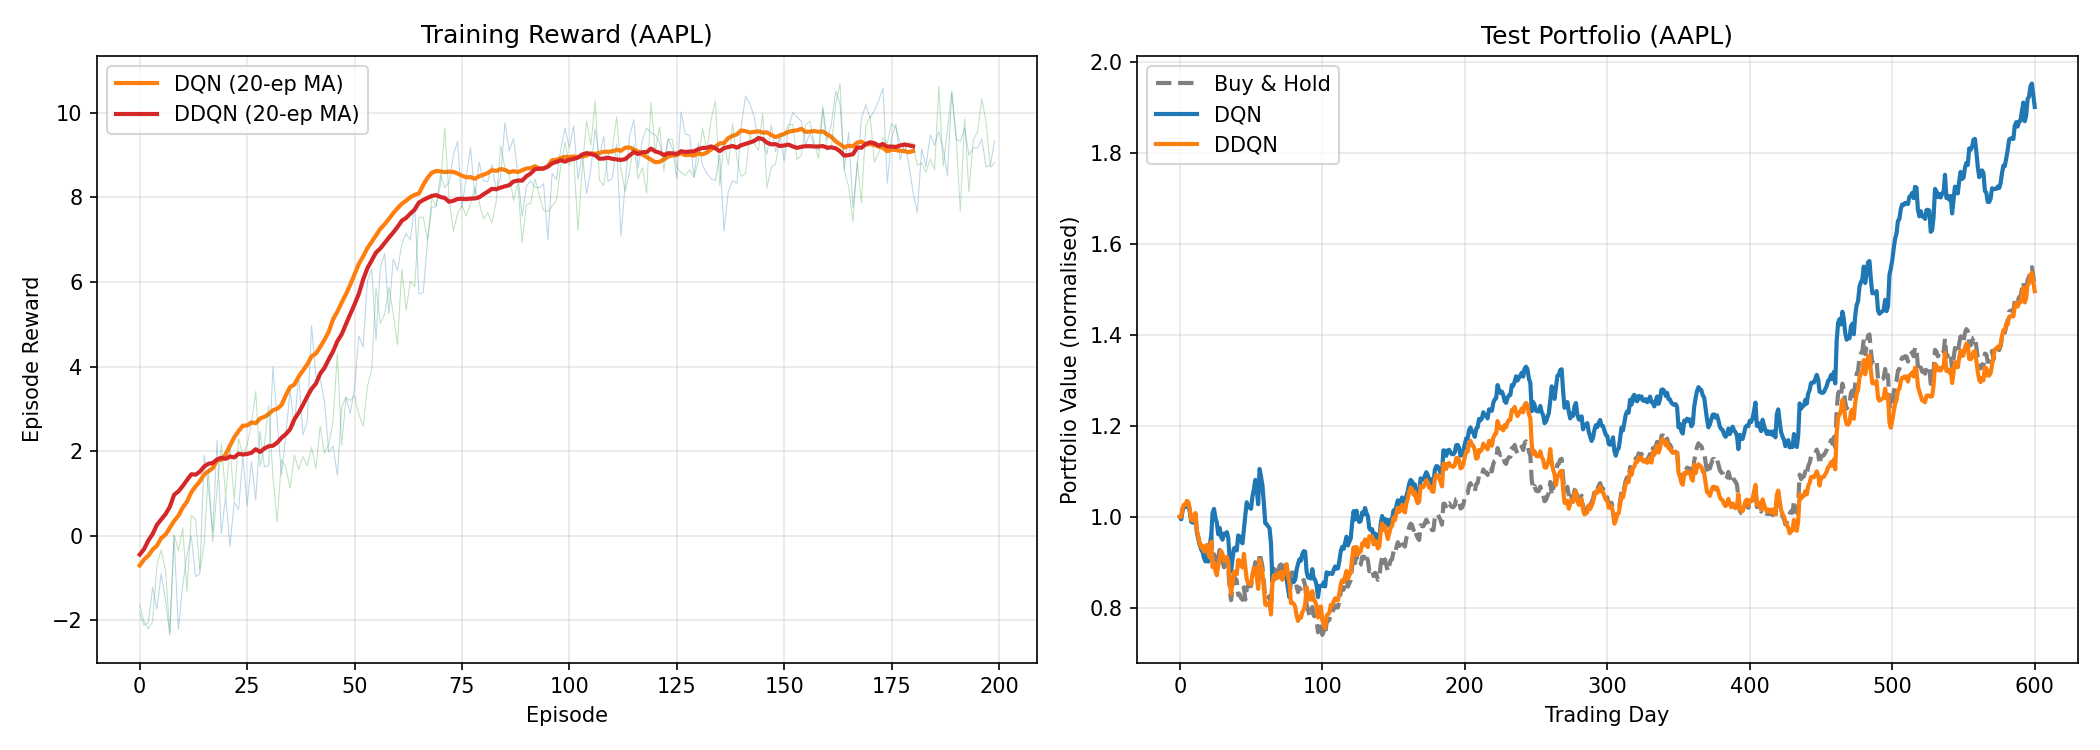
\includegraphics[width=\linewidth]{results_AAPL.png}

\vspace{-0.1em}
{\tiny \textbf{Left}: Training reward (20-ep MA). Agents generally trend upward.
\textbf{Right}: Test portfolio value. Modern RL agents (PPO, A2C, DDQN) consistently outpace Buy \& Hold.}

\vspace{0.1em}
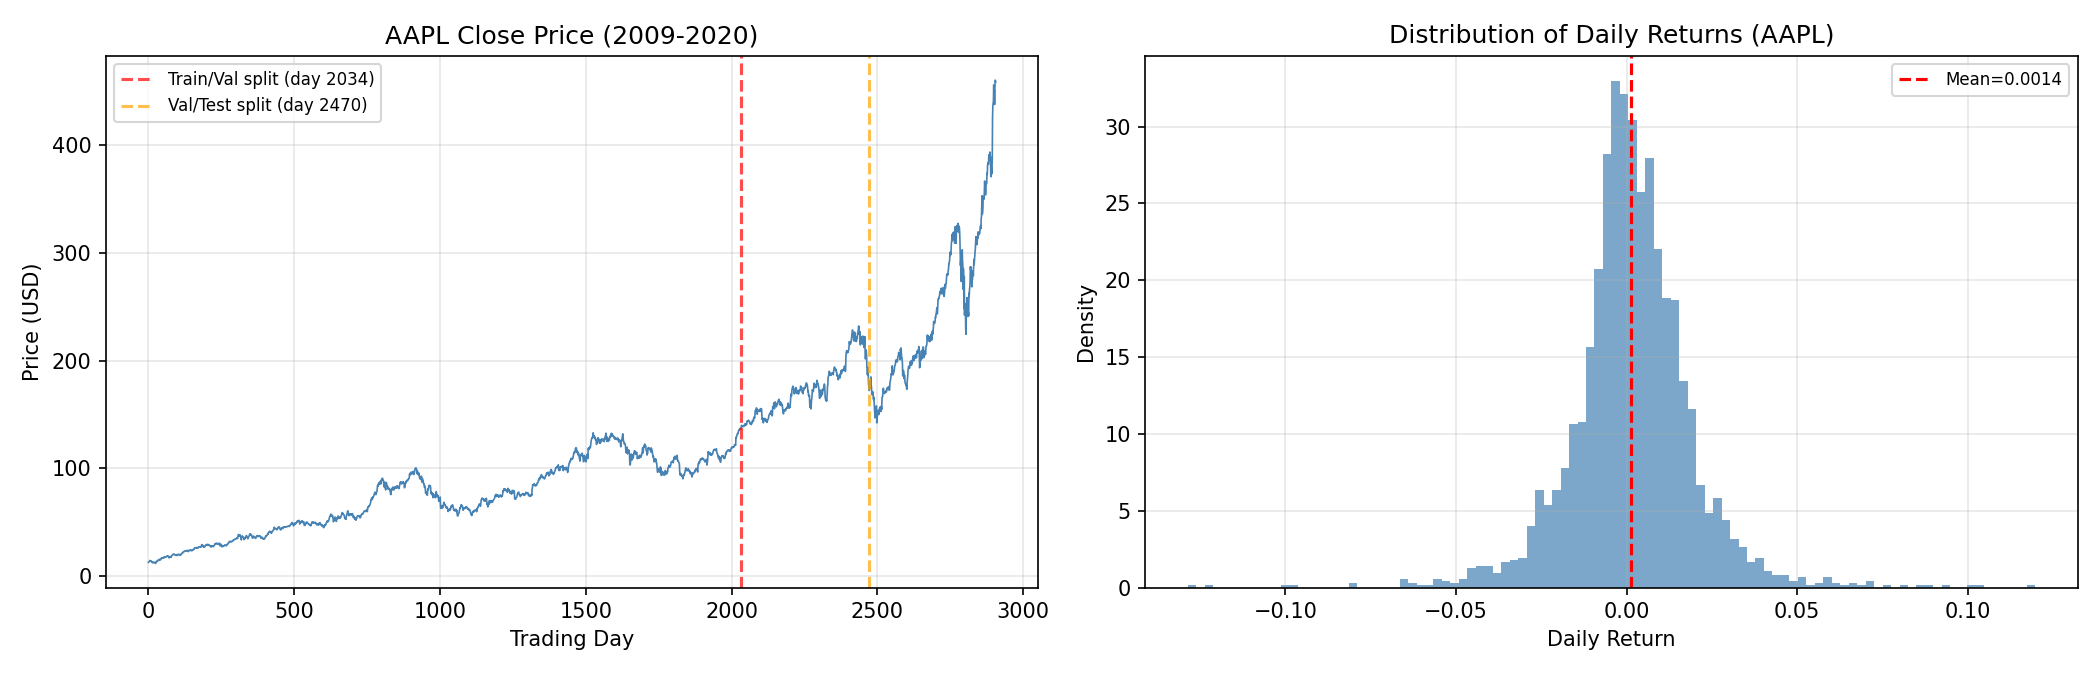
\includegraphics[width=\linewidth, height=2.6cm, keepaspectratio]{data_exploration.png}

\vspace{-0.1em}
{\tiny AAPL 2009--2020 with train/val/test splits. Test period is a strong bull market.}
\end{column}

\begin{column}{0.43\textwidth}
\vspace{-0.5em}
{\scriptsize \textbf{Test Performance:}}

\vspace{0.2em}
{\tiny
\renewcommand{\arraystretch}{1.1}
\begin{tabular}{@{}lccc@{}}
\toprule
\textbf{Model} & \textbf{Return} & \textbf{Sharpe} & \textbf{Max DD} \\
\midrule
\textcolor{accent}{PPO}   & \textcolor{good}{+184.3\%} & \textcolor{good}{2.81} & \textcolor{good}{$-16.7\%$} \\
\textcolor{accent}{A2C}   & \textcolor{good}{+182.9\%} & \textcolor{good}{2.79} & \textcolor{good}{$-17.1\%$} \\
\textcolor{accent}{DDQN}  & +172.5\% & 2.73 & \textcolor{good}{$-15.9\%$} \\
\textcolor{accent}{DQN}   & +171.7\% & 2.73 & \textcolor{good}{$-15.5\%$} \\
\textcolor{neutral}{Momentum}& +167.0\% & 2.62 & $-17.5\%$ \\
Buy \& Hold               & +159.3\% & 1.65 & $-31.4\%$ \\
ARIMA                     & +121.1\% & 1.67 & $-18.8\%$ \\
Random Forest             & +81.1\%  & 1.25 & $-26.8\%$ \\
\bottomrule
\end{tabular}}

\vspace{0.2em}
{\scriptsize \textbf{Key Takeaways:}}

\vspace{0.1em}
{\tiny
\begin{itemize}\setlength\itemsep{2pt}
  \item[\textcolor{good}{\checkmark}] \textbf{RL outperforms baselines}: All RL agents beat Buy \& Hold despite strong bull market constraints.
  \item[\textcolor{good}{\checkmark}] \textbf{Actor-Critic superiority}: PPO and A2C yield top returns, better managing noisy financial sequences.
  \item[\textcolor{good}{\checkmark}] \textbf{DDQN $\gtrsim$ DQN}: DDQN slightly outperforms DQN, consistent with reduced overestimation bias.
  \item[\textcolor{neutral}{!}] RL models exhibit lower max drawdowns ($\sim$16\%), roughly half that of B\&H.
\end{itemize}
}
\end{column}
\end{columns}
\end{frame}

\end{document}
